\chapter{Transformer Models}

\section{Overview of Transformer Model}

The Transformer model is a major breakthrough in machine learning, particularly in \textbf{Natural Language Processing (NLP)}. Introduced by Vaswani et al. in 2017 with the paper \textit{“Attention is All You Need”}, it replaced traditional recurrence-based architectures with \textbf{self-attention mechanisms}, enabling state-of-the-art performance and improved scalability.

Prior to Transformers, sequence models relied on \textbf{Recurrent Neural Networks (RNNs)}, such as \textbf{LSTMs} and \textbf{GRUs}, which processed inputs sequentially. However, they struggled with long-range dependencies, slow training due to sequential processing, and limited parallelization. Convolutional models improved efficiency but failed to capture global dependencies effectively.

The Transformer addressed these issues with \textbf{self-attention}, allowing each token to attend to all others simultaneously, eliminating sequential dependencies and enabling full parallelization. Additional innovations include \textbf{multi-head attention} for learning diverse relationships, \textbf{positional encoding} to retain order, and \textbf{feed-forward networks (FFN)} for feature transformation, along with \textbf{residual connections and layer normalization} for stable training.

Initially designed for \textbf{sequence-to-sequence tasks} like machine translation, Transformers have since revolutionized multiple domains. Models like \textbf{BERT, GPT, and T5} dominate NLP tasks, while \textbf{Vision Transformers (ViTs)} challenge CNNs in computer vision. Transformers also play a crucial role in \textbf{speech processing, multimodal learning, reinforcement learning}, and \textbf{robotics}, demonstrating their versatility.

As research continues, advancements such as \textbf{sparse attention} and \textbf{memory-efficient architectures} further enhance Transformer capabilities. With its scalability and adaptability, the Transformer remains a cornerstone of modern AI, shaping the future of deep learning.

\newpage

\section{Transformer Architecture in Detail}

The Transformer architecture, introduced in \textit{Attention Is All You Need} (Vaswani et al., 2017), is a modular and scalable design that has revolutionized sequence modeling by forgoing recurrence and convolutions in favor of a purely attention-based mechanism. Its foundational elements include tokenization, embedding, self-attention, multi-head attention, positional encoding, encoder-decoder stacks, and un-embedding layers.

\begin{figure}[H]
    \centering
    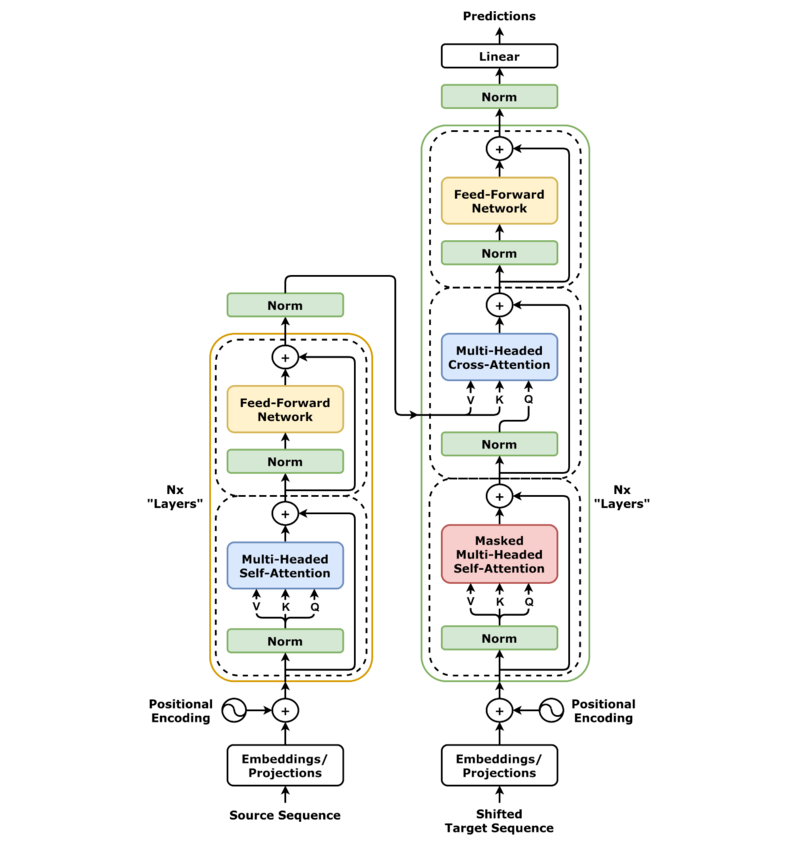
\includegraphics[width=\textwidth]{img/chap03/Transformer_architecture.png} % Adjust width as needed
    \caption{Transformer Encoder-Decoder Architecture}
    \label{fig:transformer_architecture}
\end{figure}

\subsection{Tokenization}

Before text is processed by the Transformer, it must be converted into tokens. A \textbf{tokenizer} maps segments of text (such as words, subwords, or characters) into integers from a finite vocabulary $V$ of size $n_{\text{vocab}}$. Examples of tokenization methods include Byte-Pair Encoding (BPE), WordPiece, and SentencePiece.

The input text is transformed into a token sequence:
\[
\text{``The dog barks''} \rightarrow [101, 1996, 3899, 3985, 102]
\]

Here, 101 and 102 may represent special start and end tokens.

\subsection{Embedding Layer}

The first step in a Transformer is to convert discrete token indices into continuous vector representations. This is done through a learnable \textbf{embedding layer}, which uses an embedding matrix $E \in \mathbb{R}^{n_{\text{vocab}} \times d_{\text{model}}}$, where:

\begin{itemize}
  \item $n_{\text{vocab}}$ is the size of the vocabulary,
  \item $d_{\text{model}}$ is the model dimensionality.
\end{itemize}

Each token index $t_i$ is mapped to its corresponding vector via lookup in $E$:

\[
\text{Embed}(t_i) = E[t_i] \in \mathbb{R}^{d_{\text{model}}}
\]

This can be interpreted as multiplying a one-hot vector $\mathbf{1}_{t_i} \in \mathbb{R}^{n_{\text{vocab}}}$ by the embedding matrix:

\[
\text{Embed}(t_i) = \mathbf{1}_{t_i}^\top E
\]

Embedding vectors serve as the input to the model and are updated during training to capture semantic relationships between tokens.

\subsection{Un-Embedding Layer}

At the output of the decoder (in encoder-decoder models) or the model head (in decoder-only models), we obtain hidden vectors $x \in \mathbb{R}^{d_{\text{model}}}$, which must be transformed back into the vocabulary space to compute probabilities over possible next tokens.

This is done using an \textbf{un-embedding layer}, also called the output projection layer, with weight matrix $W \in \mathbb{R}^{d_{\text{model}} \times n_{\text{vocab}}}$ and optional bias vector $b \in \mathbb{R}^{n_{\text{vocab}}}$:

\[
\text{UnEmbed}(x) = \text{softmax}(xW + b)
\]

The result is a probability distribution over all tokens in the vocabulary. Many modern Transformer implementations apply \textbf{weight tying}, where the output matrix $W$ is tied to the input embedding matrix $E$:

\[
W = E^\top
\]

This reduces the number of parameters and can improve generalization, as input and output embeddings share a common representation space.

\subsection{Positional Encoding}

Transformers process input embeddings in a permutation-invariant manner, lacking inherent order information. To encode token positions, a \textbf{positional encoding} vector is added:

\[
x_i = \text{Embed}(t_i) + \text{PosEnc}(i)
\]

where $\text{PosEnc}(i) \in \mathbb{R}^{d_{\text{model}}}$ represents the positional encoding at position $i$.

${}$\\
\textbf{Sinusoidal Positional Encoding}

The Transformer model uses a fixed sinusoidal function:

\[
\text{PosEnc}(i)_{2k} = \sin\left(\frac{i}{10000^{\frac{2k}{d_{\text{model}}}}}\right), \quad
\text{PosEnc}(i)_{2k+1} = \cos\left(\frac{i}{10000^{\frac{2k}{d_{\text{model}}}}}\right)
\]

ensuring unique encodings, relative position awareness, and generalization to unseen sequences.

${}$\\
\textbf{Complex Representation and Shift Property}

A compact formulation uses complex numbers:

\[
f(t) = \left( e^{i t / r^k} \right)_{k=0,1,\dots,d/2 -1}, \quad r = N^{2/d}
\]

where $N = 10000$. A key property is shift linearity:

\[
f(t + \Delta t) = \text{diag}(f(\Delta t)) f(t)
\]

allowing efficient matrix-based position updates.

${}$\\
\textbf{Implementation in Real-Valued Space}

Euler’s formula relates this to sine and cosine:

\[
e^{i x} = \cos x + i \sin x
\]

making real-number implementations straightforward.

${}$\\
\textbf{Example: Encoding in a 16D Space}

For $d_{\text{model}} = 16$ and $t=5$, resulting in a 16D vector:

\[
\text{PosEnc}(5)_{2k} = \sin\left(\frac{5}{10000^{2k/16}}\right), \quad
\text{PosEnc}(5)_{2k+1} = \cos\left(\frac{5}{10000^{2k/16}}\right)
\]

\subsection{Self-Attention Mechanism}

Each input vector is linearly projected into three spaces: queries $Q$, keys $K$, and values $V$:
\[
Q = XW^Q, \quad K = XW^K, \quad V = XW^V
\]

The attention weights between tokens are computed using the scaled dot-product attention:
\[
\text{Attention}(Q, K, V) = \text{softmax} \left( \frac{QK^\top}{\sqrt{d_k}} \right)V
\]

This allows the model to dynamically attend to relevant tokens within the sequence.

\subsection{Multi-Head Attention}

In Transformers, a single attention mechanism may not be sufficient to capture different relationships in the input sequence. Instead of computing attention once, the model employs multiple \textbf{attention heads}, each with its own set of projection matrices:

\[
\text{head}_i = \text{Attention}(QW_i^Q, KW_i^K, VW_i^V)
\]

where each head $i$ independently projects queries, keys, and values using learned weight matrices $W_i^Q$, $W_i^K$, and $W_i^V$.

Outputs of all attention heads are concatenated, projected using final output matrix $W^O$:

\[
\text{MultiHead}(Q, K, V) = \text{Concat} \left( \text{head}_1, \dots, \text{head}_{h} \right) W^O
\]

where:
\begin{itemize}
    \item $h$ is the number of attention heads.
    \item Each head learns a different attention pattern, allowing the model to attend to multiple aspects of the input.
    \item The final projection matrix $W^O$ ensures that the multi-head attention output remains in the original embedding space.
\end{itemize}

\begin{figure}[H]
    \centering
    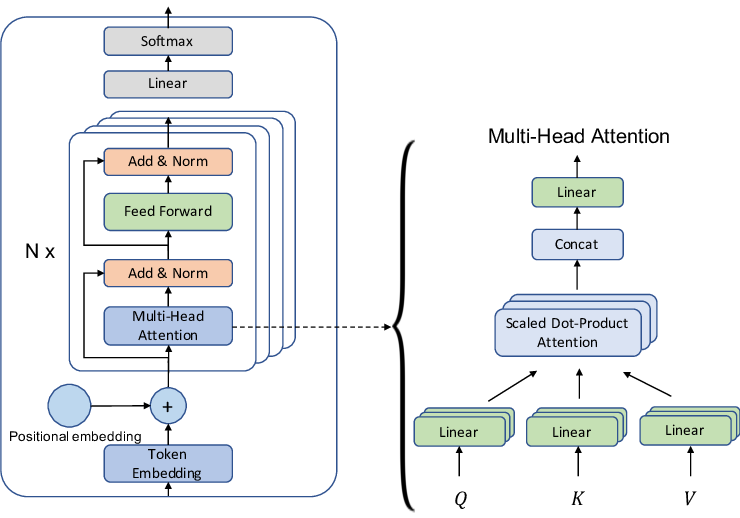
\includegraphics[width=0.7\textwidth]{img/chap03/Multiheaded.png} 
    \caption{Multiheaded attention}
    \label{fig:multi-head-attention}
\end{figure}

In practice, the embedding dimension $d_{\text{model}}$ is split across $h$ heads, with each head operating on a subspace of size $d_{\text{head}} = d_{\text{model}} / h$. For example, in GPT-2 Small:

\[
d_{\text{model}} = 768, \quad n_{\text{head}} = 12, \quad d_{\text{head}} = 64
\]

Since $12 \times 64 = 768$, the output projection matrix $W^O$ has dimensions:

\[
W^O \in \mathbb{R}^{(12 \times 64) \times 768}
\]

which ensures that the output dimension remains consistent.

This mechanism allows the Transformer to capture both local and global dependencies across different attention heads in parallel, improving expressiveness and performance.

\subsection{Feedforward Network (FFN)}

Each encoder and decoder layer contains a position-wise FFN applied independently:
\[
\text{FFN}(x) = \phi(xW^{(1)} + b^{(1)})W^{(2)} + b^{(2)}
\]
where $\phi$ is a non-linearity such as ReLU or GELU. Typically, $d_{\text{ff}} = 4d_{\text{model}}$.

\begin{figure}[H]
    \centering
    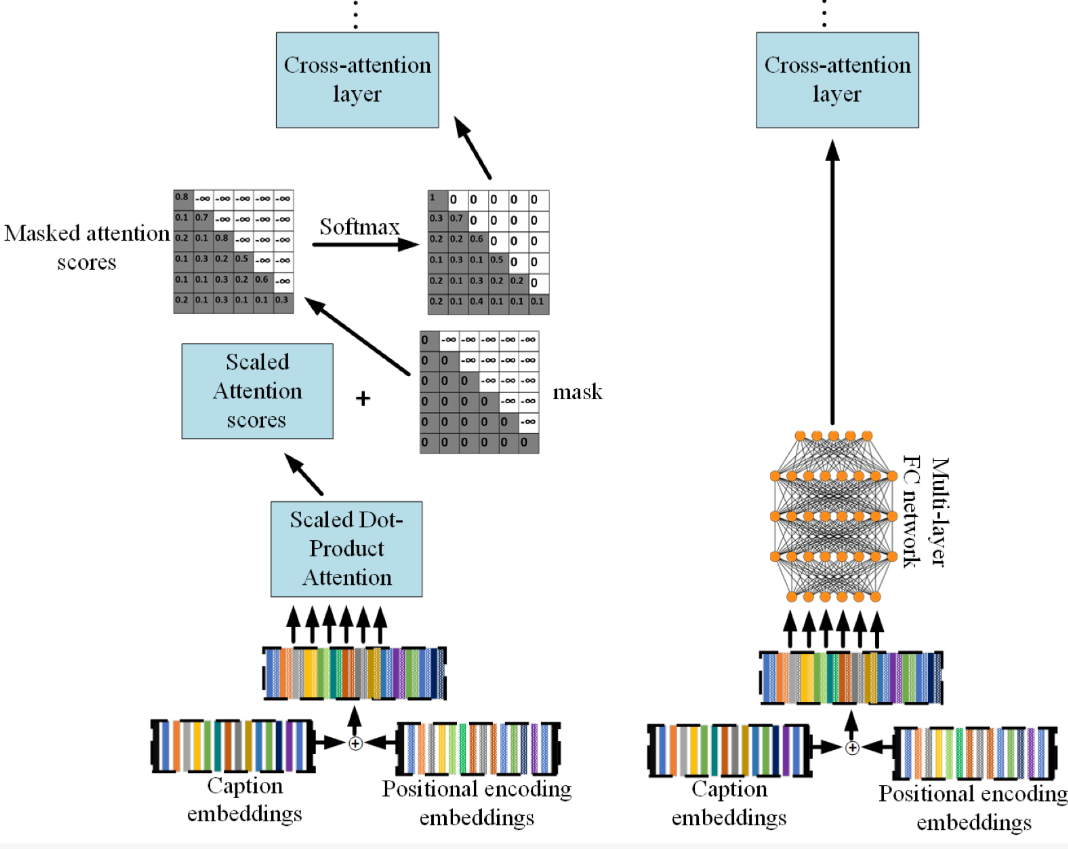
\includegraphics[width=\textwidth]{img/chap03/feed-forward.PNG} 
    \caption{The Use of Feed-Forward for Transformer Based Image Captioning Tasks}
    \label{fig:feed-forward}
\end{figure}

The figure illustrates the use of FFN and masked attention in image captioning. The left side depicts \textbf{masked attention}, where embeddings undergo scaled dot-product attention with a causal mask to maintain autoregressive properties. On the right, the \textbf{feed-forward network} refines the attended representations through a multi-layer transformation before passing them to the cross-attention layer. This enhances feature extraction and enables richer caption generation.

\subsection{Residual Connections and Layer Normalization}

Every sublayer (attention or FFN) is surrounded by a residual connection and followed (or preceded) by layer normalization (LayerNorm). Two conventions exist:

\begin{itemize}
    \item \textbf{Post-LN}: $\text{LayerNorm}(x + \text{Sublayer}(x))$
    \item \textbf{Pre-LN}: $x + \text{Sublayer}(\text{LayerNorm}(x))$
\end{itemize}

Pre-LN has been shown to stabilize training and eliminate need for learning rate warm-up.

\subsection{Encoder and Decoder Structure}

\textbf{Encoder:}

Each encoder block consists of:
\begin{enumerate}
    \item Multi-head self-attention
    \item Feed-forward network
\end{enumerate}

Each layer processes the entire sequence simultaneously using all-to-all attention.

\textbf{Decoder:}

Each decoder block consists of:
\begin{enumerate}
    \item Masked multi-head self-attention (causal)
    \item Cross-attention (to encoder outputs)
    \item Feed-forward network
\end{enumerate}

Masked attention ensures that future tokens are not visible during training.

\subsection{Masked Attention}

In Transformer decoders, masked attention ensures autoregressive token generation by preventing each token from attending to future tokens. This is achieved by adding a mask matrix $M$, which assigns $-\infty$ to positions that should not be attended to, ensuring causality before applying the softmax operation:

\[
\text{MaskedAttention}(Q, K, V) = \text{softmax} \left( M + \frac{QK^\top}{\sqrt{d_k}} \right) V
\]

where:
\begin{itemize}
    \item $Q, K, V$ are the query, key, and value matrices.
    \item $d_k$ is the key dimension.
    \item $M$ is a lower triangular matrix that blocks future tokens.
\end{itemize}

The commonly used \textbf{causal mask} is defined as:

\[
M_{\text{causal}} =
\begin{bmatrix}
0 & -\infty & -\infty & \cdots & -\infty \\
0 & 0 & -\infty & \cdots & -\infty \\
0 & 0 & 0 & \cdots & -\infty \\
\vdots & \vdots & \vdots & \ddots & -\infty \\
0 & 0 & 0 & \cdots & 0
\end{bmatrix}
\]

This mask ensures that each token can only attend to itself and past tokens, preventing information leakage from future tokens. In a non-masked attention module, $M$ is simply a matrix of zeros.

\section{Transformer Variants}

Transformers have evolved into several architectural variants, each designed for specific tasks and optimization strategies:

\begin{itemize}
    \item \textbf{Encoder-Only Models}: These architectures process the entire input sequence simultaneously, making them well-suited for tasks such as \textbf{sentence classification, named entity recognition (NER), and embedding generation}. The bidirectional nature of the encoder enables a holistic understanding of context. A prime example is \textbf{BERT}, which learns contextual representations by predicting masked tokens.
    
    \item \textbf{Decoder-Only Models}: Designed for \textbf{autoregressive generation}, these models generate tokens sequentially, conditioning each new token on previously generated ones. They are extensively used in \textbf{text generation, dialogue systems, and code synthesis}. The most prominent example is \textbf{GPT}, where decoding follows a causal attention pattern to prevent information leakage from future tokens.

    \item \textbf{Encoder-Decoder Models}: Also known as \textbf{sequence-to-sequence (seq2seq)} architectures, these models encode an input sequence into a latent representation and decode it into an output sequence. This structure is particularly effective for \textbf{machine translation, abstractive summarization, and speech-to-text conversion}. Notable examples include \textbf{T5} and \textbf{BART}, where pretraining strategies such as denoising and span prediction improve performance.

    \item \textbf{PrefixLM Models}: A hybrid approach that extends decoder-only architectures by introducing a \textbf{prefix-based masking strategy}, where certain tokens (prefix) attend to all positions while others follow causal masking. This allows for improved \textbf{controlled text generation, fill-in-the-middle tasks, and dialogue modeling}. Models like \textbf{T5 (with prefix tuning)} and \textbf{GPT-like architectures with prefix constraints} leverage this setup.
\end{itemize}

\section{Training and Pretraining Paradigms}

The effectiveness of Transformer models stems from large-scale \textbf{self-supervised pretraining}, followed by \textbf{task-specific fine-tuning}. Pretraining objectives vary based on the architecture:

\begin{itemize}
    \item \textbf{Masked Language Modeling (MLM)}: Used primarily in bidirectional encoder models like \textbf{BERT} and \textbf{RoBERTa}. In MLM, a percentage of input tokens are randomly masked, and the model is trained to predict these missing tokens based on surrounding context. This enables the model to learn deep bidirectional representations.

    \item \textbf{Autoregressive Language Modeling (AR)}: Used in decoder-only models such as \textbf{GPT}. Here, the model generates tokens sequentially, predicting the next token based on previous tokens. The training follows a left-to-right causal dependency, making it well-suited for open-ended text generation.

    \item \textbf{Prefix Language Modeling (PrefixLM)}: A hybrid approach used in models like \textbf{T5}, where a portion of the input sequence (prefix) is given full attention while subsequent tokens follow autoregressive constraints. This allows for both bidirectional understanding and controlled generation, making it useful for multitask learning.

\end{itemize}

After pretraining, these models are fine-tuned on labeled datasets for \textbf{downstream tasks} such as sentiment analysis, question answering (QA), summarization, and code generation. The fine-tuning stage involves updating model weights on task-specific objectives, often leveraging transfer learning to achieve state-of-the-art performance with limited labeled data.

\section{Advantages and Applications}

Transformers offer several advantages over previous architectures:

\begin{itemize}
    \item \textbf{No Recurrence}: Unlike RNNs or LSTMs, Transformers process input sequences in parallel, leading to faster training and inference.
    
    \item \textbf{Long-Range Dependency Modeling}: The self-attention mechanism allows direct interactions between all tokens, making it easier to capture long-range relationships.

    \item \textbf{Scalability}: Transformers can be scaled to billions of parameters and trained on large datasets across distributed systems.

    \item \textbf{Transferability}: Pretrained models serve as general-purpose language encoders and can be adapted to a wide variety of downstream tasks with minimal training data.

    \item \textbf{Multimodal Extension}: The architecture has been adapted for images (Vision Transformers), audio (e.g., Whisper), and multimodal inputs (e.g., CLIP, Flamingo).
\end{itemize}

\newpage

\section{Impacts on Natural Language Processing}

The introduction of Transformer models has profoundly transformed the field of \textbf{Natural Language Processing (NLP)}. By replacing recurrence-based architectures with self-attention mechanisms, Transformers have driven major advancements in language understanding, text generation, and multi-modal learning. Their impact extends across multiple dimensions, revolutionizing both research and real-world applications.

\subsection{Emergence of Pretrained Language Models}

Transformer-based architectures laid the foundation for a new era of \textbf{pretrained language models}, where large-scale self-supervised learning followed by task-specific fine-tuning became the dominant paradigm. Pretrained Transformers learn rich representations from massive text corpora and transfer this knowledge to a wide range of NLP tasks.

\begin{itemize}
    \item \textbf{BERT (Bidirectional Encoder Representations from Transformers)} introduced bidirectional attention, allowing models to learn deep contextual representations. Pretraining tasks such as \textbf{Masked Language Modeling (MLM)} and \textbf{Next Sentence Prediction (NSP)} enabled BERT to outperform previous methods on benchmarks like GLUE and SQuAD.

    \item \textbf{GPT (Generative Pre-trained Transformer)} adopted an \textbf{autoregressive} training approach, using causal masking to predict the next token in a sequence. Unlike BERT, GPT models only use the decoder portion of the Transformer and excel at \textbf{unstructured text generation, dialogue modeling, and code synthesis}. GPT-3, with its 175 billion parameters, demonstrated unprecedented capabilities in few-shot and zero-shot learning.

    \item \textbf{T5 (Text-to-Text Transfer Transformer)} unified NLP tasks into a \textbf{single sequence-to-sequence framework}, converting tasks such as classification, summarization, and translation into text generation problems. This approach enabled greater flexibility and improved generalization across diverse NLP challenges.

    \item \textbf{RoBERTa, XLNet, ALBERT, and ELECTRA} introduced optimizations to Transformer training, improving efficiency, sample efficiency, and generalization.
\end{itemize}

\subsection{State-of-the-Art Performance on NLP Benchmarks}

Transformer-based models have consistently set new records on NLP leaderboards by achieving superior results across various benchmarks:

\begin{itemize}
    \item \textbf{Question Answering}: BERT and T5 have dramatically improved performance on datasets like \textbf{SQuAD} and \textbf{Natural Questions}, surpassing human-level accuracy in some cases.
    \item \textbf{Named Entity Recognition (NER)}: Transformers have achieved near-human accuracy on entity recognition benchmarks such as \textbf{CoNLL-2003}.
    \item \textbf{Machine Translation}: Models like \textbf{mBART}, \textbf{MarianMT} have improved translation quality by leveraging Transformer architectures trained on multilingual data.
    \item \textbf{Text Summarization}: Sequence-to-sequence Transformers like \textbf{PEGASUS} and \textbf{BART} produce highly coherent and human-like summaries.
    \item \textbf{Sentiment Analysis and Text Classification}: Fine-tuned Transformer models outperform traditional RNN/CNN approaches on sentiment datasets such as \textbf{IMDB} and \textbf{Yelp Reviews}.
    \item \textbf{Text Generation}: Large autoregressive models such as \textbf{GPT-3} and \textbf{ChatGPT} have demonstrated advanced capabilities in free-form text generation and reasoning.
\end{itemize}

The ability to fine-tune these models with minimal labeled data has led to a major shift in how NLP tasks are approached, making \textbf{transfer learning} the standard technique for both academia and industry.

\subsection{Contextualized Word Representations}

Unlike traditional word embedding methods such as \textbf{Word2Vec} and \textbf{GloVe}, which assign static vectors to words, Transformer-based models generate \textbf{contextualized embeddings}, where representation of a word changes based on its surrounding context. This allows for:
\begin{itemize}
    \item \textbf{Disambiguation of polysemous words}: The meaning of words like \textit{bank} (financial institution vs. riverbank) is inferred dynamically.
    \item \textbf{Better syntactic and semantic understanding}: Context-aware embeddings improve tasks such as \textbf{coreference resolution} and \textbf{semantic role labeling}.
    \item \textbf{Stronger generalization}: Models trained with contextual embeddings outperform static embedding models across diverse NLP tasks.
\end{itemize}

\subsection{Scalability and Parallelization}

The Transformer’s ability to process entire sequences in parallel (due to the absence of recurrent dependencies) has enabled the training of extremely large-scale models. Unlike RNNs, which process tokens sequentially, Transformers leverage \textbf{self-attention} and \textbf{matrix multiplications}, making them highly parallelizable on modern hardware such as GPUs and TPUs. This has led to:

\begin{itemize}
    \item The emergence of massive models such as \textbf{GPT-3 (175B parameters)} and \textbf{PaLM (540B parameters)}.
    \item Training on web-scale datasets, enabling few-shot and zero-shot generalization capabilities.
    \item Faster inference times and efficiency improvements through optimizations like \textbf{sparse attention} and \textbf{mixture of experts (MoE)} architectures.
\end{itemize}

\subsection{Cross-Lingual and Multilingual Learning}

Transformers have significantly advanced multilingual NLP, enabling models to generalize across languages with minimal or no supervision. \textbf{Multilingual BERT (mBERT)} and \textbf{XLM-RoBERTa} have demonstrated the ability to:
\begin{itemize}
    \item Transfer knowledge between languages, allowing zero-shot learning on low-resource languages.
    \item Improve translation, multilingual document classification, and cross-lingual retrieval.
    \item Enhance speech and text-based applications in non-English languages.
\end{itemize}

\subsection{Transformers Beyond NLP}

Although originally designed for NLP, Transformer-based architectures have inspired advancements in multiple domains:

\begin{itemize}
    \item \textbf{Computer Vision}: \textbf{Vision Transformers (ViTs)} apply self-attention mechanisms to image patches, outperforming CNNs on classification tasks and challenging traditional vision models.
    \item \textbf{Speech Processing}: Self-supervised models like \textbf{Wav2Vec} and \textbf{HuBERT} apply Transformer-based architectures to learn representations from raw audio, improving speech recognition systems.
    \item \textbf{Reinforcement Learning and Robotics}: Transformers have been applied to decision-making and planning tasks in reinforcement learning (\textbf{Decision Transformer}) and robotic control.
    \item \textbf{Multimodal Learning}: Models like \textbf{CLIP}, \textbf{DALL·E}, \textbf{Flamingo} integrate visual and textual modalities, enabling text-to-image generation and image-based reasoning.
\end{itemize}

\subsection{Ethical Considerations and Challenges}

Despite their successes, Transformer-based models introduce several challenges:
\begin{itemize}
    \item \textbf{Computational Costs}: Training large Transformers requires significant energy and hardware resources.
    \item \textbf{Bias and Fairness}: Pretrained models inherit biases from their training data, necessitating research on bias mitigation techniques.
    \item \textbf{Interpretability}: The complexity of self-attention mechanisms makes it difficult to explain model decisions.
    \item \textbf{Misinformation and Abuse}: Powerful generative models pose risks in generating deceptive or harmful content.
\end{itemize}

Addressing these concerns remains a crucial focus of ongoing research in NLP.

\section{Conclusion}

The \textbf{Transformer} model has fundamentally reshaped the landscape of \textbf{Natural Language Processing (NLP)} and beyond. Introduced as an alternative to recurrent and convolutional architectures, the Transformer’s \textbf{self-attention mechanism} has enabled unprecedented advancements in sequence modeling by allowing parallel computation, long-range dependency capture, and efficient scaling.

Through the emergence of \textbf{pretrained language models} such as \textbf{BERT, GPT, T5, and their successors}, Transformers have established a new standard for \textbf{transfer learning}, drastically reducing the amount of task-specific labeled data needed for fine-tuning. These models have achieved state-of-the-art performance in \textbf{text generation, machine translation, question answering, summarization, sentiment analysis}, and many other tasks. Furthermore, the ability of Transformers to generate \textbf{contextualized word representations} has led to more robust and semantically aware NLP systems compared to static embedding methods.

The scalability of Transformer models, facilitated by their \textbf{parallelizable architecture}, has paved the way for training extremely large-scale models with billions of parameters. The impact of such models extends beyond NLP, influencing fields such as \textbf{computer vision, speech processing, reinforcement learning, and multimodal AI}. Vision Transformers (ViTs) have challenged the dominance of convolutional neural networks, while models like \textbf{CLIP and DALL·E} showcase the potential of multimodal learning.

Despite their remarkable achievements, Transformers also present challenges. Their immense \textbf{computational requirements} raise concerns about accessibility and sustainability, while issues related to \textbf{bias, interpretability, and ethical considerations} remain key areas of active research. Ensuring responsible deployment of these powerful models is crucial as they continue to shape the future of AI.

Looking ahead, research in \textbf{efficient Transformers, sparse attention mechanisms, knowledge distillation, and low-resource adaptation} will play a critical role in making these models more accessible, scalable, and interpretable. With continuous advancements, the Transformer architecture remains a cornerstone of modern AI, driving innovations that push the boundaries of natural language understanding and generation.

\newpage 